% Lineal regression 
\begin{frame}{Definition of linear regression}
    \section{Linear regression}  
    \subsection{Definition of linear regression}
    Basic definition of a lineal model: 
      \begin{equation}
        y(x,w) = x \cdot w^T
      \end{equation}
      where $x \in \{1\}\times\R^{d}$ and $w \in \R^{d+1}$. 
  \end{frame}
  
  \begin{frame}{Problems of global polinomial function}
    \subsection{Some problems}
    \textbf{Runge's phenomenon}\footnote{Sources: 
    General overview of approximation theory \cite{ACourseInApproximationTheory} 
    and Wikipedia \cite{Splines} and \cite{RungePhenomenon}}
    \begin{figure}
      \centering
      \begin{subfigure}[b]{0.4\textwidth}
          \centering
          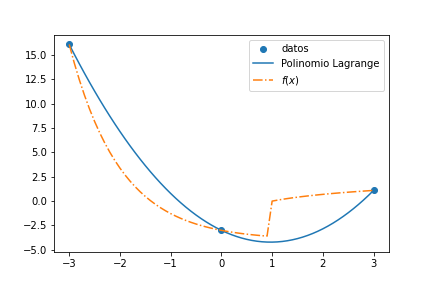
\includegraphics[width=\textwidth]{02_Lineal_models/lagrange-3-datos.png}
          \caption[]%
          {{\small Lagrange polynomial of three nodes}}    
          \label{fig:mean and std of net14}
      \end{subfigure}
      \hfill
      \begin{subfigure}[b]{0.4\textwidth}   
          \centering 
          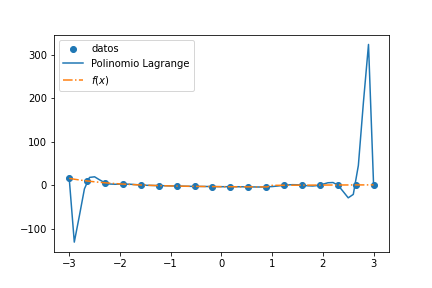
\includegraphics[width=\textwidth]{02_Lineal_models/lagrange-18-datos.png}
          \caption[]%
          {{\small Lagrange polynomial of 18 nodes}}    
          \label{fig:}
      \end{subfigure}
      \caption[ The error converges to infinity]
      {\small The error converges to infinity} 
      \label{fig:01errorToInfinty}
    \end{figure}
  \end{frame}
  
  \begin{frame}{Explantation}
    Runge's phenomenon is the consequence of two properties of this problem: 
    \begin{enumerate}
      \item   The magnitude of the n-th order derivatives of this particular function grows quickly when n increases.
      \item   The equidistance between points leads to a Lebesgue constant that increases quickly when n increases. \footnote{Source: \cite{LebesgueConstant}} (Lagrange Base Polynomial)
    \end{enumerate}
  
    Solutions: 
    \begin{enumerate}
      \item Controlling derivatives: \textbf{Splines} (Solve 1).
      \item Reducing the domain where a variable could effect \textbf{basic functions}(Solve 2).
    \end{enumerate}
  
    More aproachs??? \textcolor{red}{I need to read \cite{ACourseInApproximationTheory}}
  \end{frame}
  
  \begin{frame}
    \frametitle{Generalization of lineal models}
    \subsection{Generalization by basic functions}
    It can be generalized as: 
      \begin{equation}
        y(x,w) = \phi(x) \cdot w^T
      \end{equation}
      where $\phi_j(x)$ are known as \textbf{basic functions}. 
  
      (Notation: $\phi_0(x) = w_0$ is usually known as \textbf{bias}). 
  
  \end{frame}
  
  \begin{frame}
    \frametitle{Some values of basic functions}
    \begin{center}
      \begin{tabular}{ |c| c| c |}
        \hline
       Gaussian & Logistic sigmoid & Wavelets\footnote{Read more at 
       \cite{Wavelet} and \cite{ACourseInApproximationTheory}} \\ 
       \hline
       $exp \left(-\frac{(x-\mu)^2}{2 \sigma^2}\right)$
       & % Sigmoid formula
       $\frac{1}{1 + \exp(\frac{x-\mu}{\sigma})}$  
      & $c \sum (-1)^i \sin(2^i \pi x)$ \\  
       % images 
       % 1. Gaussian
       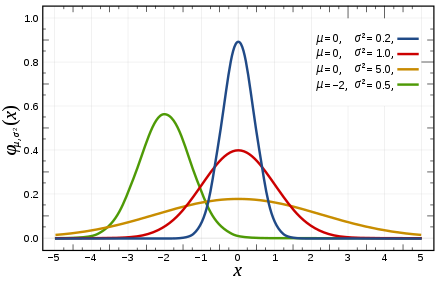
\includegraphics[width=.3\textwidth]{02_Lineal_models/gaussian_function.png}
        & % 2. Sigmoid function 
        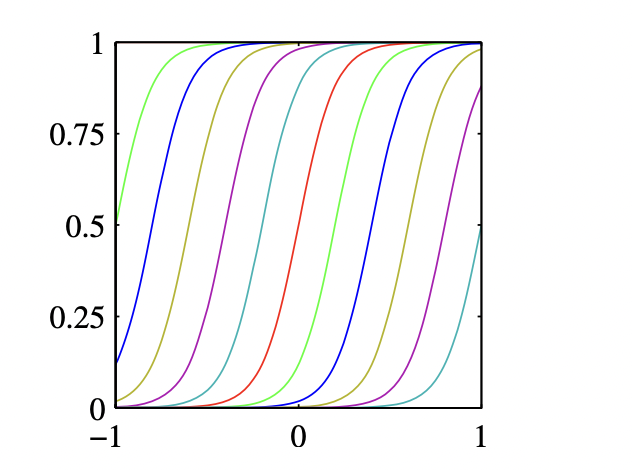
\includegraphics[width=.3\textwidth]{02_Lineal_models/sigmoid_function.png}
        & 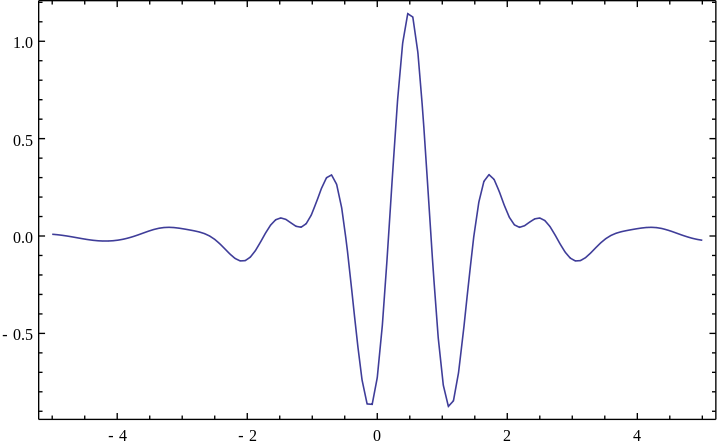
\includegraphics[width=.3\textwidth]{02_Lineal_models/MeyerMathematica.png} \\
       \hline  
      \end{tabular}
      \end{center}
  \end{frame}
  
  \begin{frame}
    \frametitle{Least Squares}
    \section{Least Squares}
    How good is our approximation?
  
    We also showed that this error function could 
    be motivated as the maximum likelihood 
    solution under an assumed Gaussian noise model.
  \end{frame}
  
  \begin{frame}{Maximum likelihood and least squares}
    \subsection{Maximum likelihood deduction}
    The error function least squared could be motivated
    al the maximum likelihood solution. 
  
    \begin{equation}
      t = y(x,w) + \epsilon 
    \end{equation}
    where $\epsilon \sim \mathcal{N}(0, \beta^{-1})$ 
    and $\beta \in \R$ is the precision ($\beta^{-1} = \sigma^2$). 
  
    Thus we can write
    % la probabilidad t a partir de x es 
    %  igual a la probabilidad de que t lo sea a partir de la normal
    % abuso de notación N
    % N es la función de probabilidad de una normal 
    % de media y y de varianza la inversa de la precisión 
    \begin{equation}
      p(t | x, w, \beta) = \mathcal{N}(t | y(x,y), \beta^{-1}). 
    \end{equation}
  
    \begin{equation}
      \mathbb{E}[t | x] = 
      \int t p(t|x) dt
      = y(x,w).
    \end{equation}
    
  \end{frame}
  
  \begin{frame}
    Set of inputs $X = \{x_i\}_{1\leq i < n}$, and their targets $\{ t_i\}_{1\leq i < n}$. 
    So we obtain the following expression for the likelihood function, which is a function adjustable parameters $w$ and $\beta$. 
  
    % nuestra función y(x,w) es ahora un modelo lineal
    \begin{equation}
      p (t | X, w, \beta) = 
      \prod^{n}_{i=1} 
      \mathcal{N}(t_i | w^t \phi(x_i), \beta^{-1})
    \end{equation}
    Taking logarithm of the likelihood function and using the standard form for the univariate Gaussian
  \end{frame}
  \begin{frame}
    For a single real-valued variable x, the Gaussian distribution is defined by
  
    \begin{equation}
      \mathcal{N}(x | \mu, \sigma^2) 
      = 
      \frac{1}{\sqrt{2 \pi \sigma^2}}
      \exp 
      \left\{
        - \frac{1}{2 \sigma^2} (x - \mu)^2
      \right\}. 
    \end{equation}
  
    We have
    \begin{equation}
      \log p(t|X,w, \beta) 
      =
      \sum^n_{i=1}
      % first fraction 
      = \frac{n}{2} \log \beta 
      - \frac{n}{2} \log  
      - \frac{n \beta}{2} 
      \sum_{i = 1}^n
      (t_i - w^T \phi(x_i))^2.
    \end{equation}
  
    Maximum likelihood for $w$ and $\beta$.
  
    Where is a maximum? 
  
    Notice that $\beta > 0$ by definition of variance. 
    The addend where $w$ appears,  are negative parabolas. 
  \end{frame}
  
  \begin{frame}
    \begin{align}
      \nabla_w \log p(t|X,w, \beta) 
      &= 
      \nabla_w 
      \left\{ 
        - \frac{1}{2} 
        \sum_{i = 1}^n
        (t_i - w^T \phi(x_i))^2
      \right\}
      \\
      &= 
      \sum _{i=1}^n
      (t_i - w^T \phi(x_i))
      \phi(x_i)^T.
    \end{align}
  
    Setting this gradient to zero gives 
  
    \begin{equation}
      0 
      = 
      \sum_{i = 0}^n
      t_i \phi(x_i)^T
      - 
      w^T
      \left(
        \sum_{i=1}^n
        \phi(x_i)
        \phi(x_i)^T
      \right)
    \end{equation}
  \end{frame}
  
  \begin{frame}
    Writing as a matrix 
  
    \begin{equation}
      \Phi = \{ \phi_c(x_r)\}_{
          \substack{ 
            0 \leq c < m\\
            1 \leq r \leq n
          }
      },
    \end{equation}
    where $m$ of the models $\phi: \R^d \longrightarrow \R^M$. 
  
    Solving for $w$ we obtain 
  
    \begin{equation}
      w = 
      \left(
        \Phi^T \Phi
      \right)^{-1}
      \Phi^T t.
    \end{equation}
    
  \end{frame}
  
  \begin{frame}{Definition Moore-Penrose pseudo-inverse}
    \subsection{Definition Moore-Penrose pseudo-inverse}
    \begin{definition}
      \textbf{Moore-Penrose pseudo-inverse}
    \begin{equation}
      \Phi^\dagger 
      = 
      \left(
        \Phi^T \Phi
      \right)^{-1}
      \Phi^T
    \end{equation}
  \end{definition}
    Properties
    \begin{itemize}
      \item Generalization of the notion of inverse to non square matrices.
      \item If $\Phi$ is square and invertible then $\Phi^\dagger =  \Phi^{-1}$. 
    \end{itemize}
  \end{frame}
% Minimizing the squared error
\begin{frame}{Minimizing squared error}
    Let $L(t, y(x)) = (y(x)-t)^2$ the squared loss function. 
    For which $y$ the error is minimum?
    \begin{equation}
       \E [L] = 
       \int \int 
       L(x,y ) p(x,t)
       dx dt 
       = 
       \int \int 
       (y(x)-t)^2 p(x,t)
       dx dt
    \end{equation}
    If we assume a completely flexible function, we can do this formally using the calculus of variations to give

    \begin{equation}
        \frac{\partial \E[L]}{\partial y(x)}
        = 
        2 \int 
            (y(x)-t)p(x,t) dt
        = 0
    \end{equation}
\end{frame}

  \begin{frame}{The optimal prediction}
    \subsection{The optimal prediction}
    Solving for $y(x)$, and using the sum and product rules of probability, we obtain
    \begin{equation}
        y(x)
        = 
        \frac{1}{p(x)} 
        \int t p(x,t) dt
        = 
        \int t p(t|x) dt
        = \E_t[t|x].
    \end{equation}

    
    \textbf{The optimal prediction for a deterministic}, denotes by $h(x)$, is given by 
    \begin{equation}
      h(x) = \E [t|x] = \int t p(t|x) dt.
    \end{equation}
  \end{frame}

  \begin{frame}{Fixing an objective function}
  Why our goal is $\E [t|x]$ instead of $p(x,t)$?
   
  Transformation: 
  \begin{enumerate}
    \item Consider a domain for $x$ and $t$.
    \item Change $y(x)$ for $y(x,t)$.
    \item For training 
    \begin{equation}
        \hat y (x,y) = \frac{\#\{(a,b) \in \mathcal{D} : (a,b) = (x,y)\}}{ \#D}
    \end{equation}
  \end{enumerate}

  Answer 
  \begin{itemize}
    \item The new training data set got shrunken, 
    since where we got redundance now we got one frequency.
    \item \textbf{The probability of a point in a space is zero!!!}
  \end{itemize}
  \textcolor{red}{So this approach only have sense at classification problems}. 
  \end{frame}

